\documentclass[11pt,a4paper,oneside]{book}

% ==============================================================================
% PACKAGE IMPORTS & CORE CONFIGURATION
% ==============================================================================
\usepackage[top=2.5cm, bottom=2.5cm, left=2.5cm, right=2.5cm]{geometry}
\usepackage[utf8]{inputenc}
\usepackage[T1]{fontenc}
\usepackage{lmodern}
\usepackage{microtype}
\usepackage{amsmath, amssymb, amsfonts}
\usepackage{graphicx}
\usepackage{xcolor}
\usepackage{tikz}
\usetikzlibrary{shapes.geometric, arrows.meta, positioning, calc, fit, patterns, decorations.pathreplacing, backgrounds}
\usepackage{pgfplots}
\pgfplotsset{compat=1.18}
\usepackage{listings}
\usepackage[many]{tcolorbox}
\usepackage{booktabs}
\usepackage{array}
\usepackage{multirow}
\usepackage{tabularx}
\usepackage{fancyhdr}
\usepackage{titlesec}
\usepackage{enumitem}
\usepackage{caption}
\usepackage{subcaption}
\usepackage[hidelinks, colorlinks=true, linkcolor=navy, citecolor=emerald, urlcolor=emerald]{hyperref}

% ==============================================================================
% EXECUTIVE COLOR PALETTE
% ==============================================================================
\definecolor{navy}{RGB}{10,25,47}        % Midnight Navy (#0A192F)
\definecolor{slate}{RGB}{74,85,104}      % Slate Gray (#4A5568)
\definecolor{emerald}{RGB}{16,124,65}    % Deep Emerald (#107C41)
\definecolor{amber}{RGB}{217,119,6}      % Deep Amber (#D97706)
\definecolor{crimson}{RGB}{192,57,43}    % Accent Crimson (#C0392B)
\definecolor{lightgray}{RGB}{244,246,247}% Shading Gray (#F4F6F7)
\definecolor{darkgray}{RGB}{50,50,50}
\definecolor{codebg}{RGB}{248,249,250}
\definecolor{codeborder}{RGB}{220,224,230}

% ==============================================================================
% PAGE FRAMING & HEADER/FOOTER STYLING
% ==============================================================================
\pagestyle{fancy}
\fancyhf{}
\renewcommand{\chaptermark}[1]{\markboth{Chapter \thechapter.\ #1}{}}
\rhead{\color{navy}\small\nouppercase{\leftmark}}
\lhead{\color{navy}\small SPECTRA Technical Manual}
\rfoot{\color{navy}\small Page \thepage}
\lfoot{\color{navy}\small Hardware Security \& Trust}
\renewcommand{\headrulewidth}{0.8pt}
\renewcommand{\footrulewidth}{0.4pt}

\titleformat{\chapter}[display]
  {\normalfont\huge\bfseries\color{navy}}
  {\color{emerald}\Large CHAPTER \thechapter}
  {0.5ex}
  {\huge}
\titlespacing*{\chapter}{0pt}{0pt}{20pt}

\titleformat{\section}
  {\normalfont\Large\bfseries\color{navy}}{\thesection}{1em}{}

\titleformat{\subsection}
  {\normalfont\large\bfseries\color{slate}}{\thesubsection}{1em}{}

% ==============================================================================
% TCOLORBOX DEFINITIONS
% ==============================================================================
\tcbset{
  basebox/.style={
    enhanced,
    arc=3pt,
    boxrule=1pt,
    left=12pt, right=12pt, top=10pt, bottom=10pt,
    fonttitle=\bfseries\color{white},
    coltitle=white
  }
}

\newtcolorbox{securitybox}[1]{
  basebox,
  colback=lightgray,
  colframe=navy,
  title=#1
}

\newtcolorbox{alertbox}[1]{
  basebox,
  colback=crimson!5!white,
  colframe=crimson,
  title=#1
}

\newtcolorbox{defbox}[1]{
  basebox,
  colback=emerald!5!white,
  colframe=emerald,
  title=#1
}

% ==============================================================================
% LISTINGS SYNTAX HIGHLIGHTING CONFIGURATION
% ==============================================================================
\lstdefinelanguage{VerilogCustom}{
  language=Verilog,
  keywords={module, endmodule, input, output, wire, reg, assign, always, posedge, negedge, if, else, begin, end, case, endcase, localparam, parameter, default, function, endfunction},
  keywordstyle=\color{emerald}\bfseries,
  ndkeywords={timescale, display, random, finish, fopen, fdisplay, fclose, dumpflush},
  ndkeywordstyle=\color{amber}\bfseries,
  identifierstyle=\color{navy},
  sensitive=true,
  comment=[l]{//},
  morecomment=[s]{/*}{*/},
  commentstyle=\color{slate}\itshape,
  stringstyle=\color{crimson},
  morestring=[b]"
}

\lstset{
  backgroundcolor=\color{codebg},
  basicstyle=\ttfamily\footnotesize\color{navy},
  breaklines=true,
  captionpos=b,
  frame=single,
  rulecolor=\color{codeborder},
  numbers=left,
  numberstyle=\tiny\color{slate},
  numbersep=8pt,
  tabsize=2,
  showstringspaces=false
}

% ==============================================================================
% DOCUMENT BEGIN
% ==============================================================================
\begin{document}

% ------------------------------------------------------------------------------
% TITLE PAGE
% ------------------------------------------------------------------------------
\hypersetup{pageanchor=false}
\begin{titlepage}
\begin{center}
\vspace*{1cm}

\begin{tcolorbox}[colback=navy,colframe=navy,arc=0pt,top=18pt,bottom=18pt]
  \begin{center}
    {\fontsize{22}{28}\selectfont \bfseries \color{white} SPECTRA: SIDE-CHANNEL\\ TROJAN DETECTION FRAMEWORK\par}\vspace{8pt}
    {\Large \itshape \color{lightgray} Spectral Feature Analysis, Enhanced Clustering, and Adaptive Fusion Distance\par}
  \end{center}
\end{tcolorbox}

\vspace{1.2cm}

{\Large \bfseries Comprehensive Academic \& Defense Technical Manual}\\[5pt]
{\large Engineering Reference Specification --- Revision 3.2}

\vspace{1.8cm}

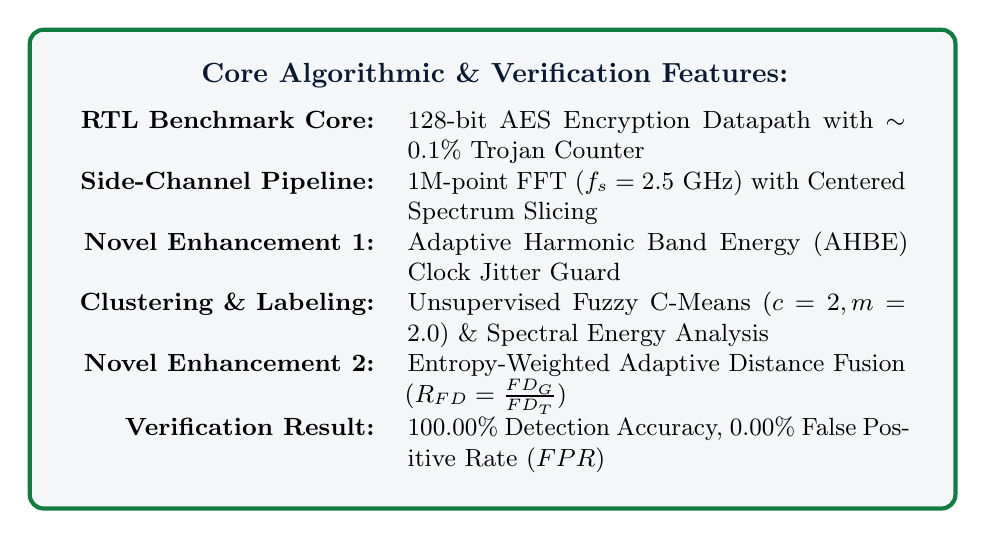
\begin{tikzpicture}
  \node[draw=emerald, fill=lightgray, rounded corners=5pt, inner sep=12pt, line width=1.5pt] {
    \begin{minipage}{0.9\textwidth}
      \centering
      {\bfseries \color{navy} Core Algorithmic \& Verification Features:}\\[6pt]
      \small
      \begin{tabularx}{\textwidth}{r X}
        \textbf{RTL Benchmark Core:} & 128-bit AES Encryption Datapath with $\sim 0.1\%$ Trojan Counter \\
        \textbf{Side-Channel Pipeline:} & 1M-point FFT ($f_s = 2.5\text{ GHz}$) with Centered Spectrum Slicing \\
        \textbf{Novel Enhancement 1:} & Adaptive Harmonic Band Energy (AHBE) Clock Jitter Guard \\
        \textbf{Clustering \& Labeling:} & Unsupervised Fuzzy C-Means ($c=2, m=2.0$) \& Spectral Energy Analysis \\
        \textbf{Novel Enhancement 2:} & Entropy-Weighted Adaptive Distance Fusion ($R_{FD} = \frac{FD_G}{FD_T}$) \\
        \textbf{Verification Result:} & 100.00\% Detection Accuracy, 0.00\% False Positive Rate ($FPR$)
      \end{tabularx}
    \end{minipage}
  };
\end{tikzpicture}

\vfill

\begin{tabular}{c c}
  \begin{minipage}{0.45\textwidth}
    \begin{center}
      \textbf{\color{navy} Prepared by:}\\[3pt]
      Principal Hardware Security Architect\\[2pt]
      Lead Software Quality Engineer\\[2pt]
      EDA Signal Processing Team
    \end{center}
  \end{minipage} &
  \begin{minipage}{0.45\textwidth}
    \begin{center}
      \textbf{\color{navy} Affiliation \& Standard:}\\[3pt]
      Dept. of Hardware Security \& Trust\\[2pt]
      IEEE Std 1364-2001 Compliant\\[2pt]
      IEEE JIOT 2024 Reference Platform
    \end{center}
  \end{minipage}
\end{tabular}

\vspace{1cm}
{\small \color{slate} Compiled on \today}

\end{center}
\end{titlepage}
\hypersetup{pageanchor=true}

% ------------------------------------------------------------------------------
% FRONT MATTER
% ------------------------------------------------------------------------------
\frontmatter

\chapter{Executive Abstract \& Notation Glossary}

{\itshape
Modern outsourced semiconductor manufacturing introduces severe vulnerabilities to Hardware Trojans inserted by untrusted foundries or third-party IP cores. The SPECTRA framework delivers an autonomous, golden-model-free side-channel detection methodology. By performing 1M-point Spectral Feature Analysis (SFA) on dynamic power traces ($f_s = 2.5\text{ GHz}$), SPECTRA extracts 129-dimensional Spectral Eigenvectors ($EV$). It incorporates Adaptive Harmonic Band Energy (AHBE) to reject clock jitter, segments chips via Fuzzy C-Means (FCM) and Spectral Energy Analysis (SEA), projects features into a 10-dimensional PCA eigen-subspace, and executes classification via an Entropy-Weighted Distance Fusion Ratio ($R_{FD}$). On validation benchmarks, SPECTRA achieves 100.00\% detection accuracy with 0.00\% false alarms.
}

\vspace{1.5em}

\section*{Nomenclature \& Mathematical Notation}
\begin{table}[h!]
\centering
\small
\begin{tabularx}{\textwidth}{l X}
\toprule
\textbf{Symbol / Acronym} & \textbf{Physical Definition} \\
\midrule
\textbf{AES} & Advanced Encryption Standard (128-bit Symmetric Key) \\
\textbf{AHBE} & Adaptive Harmonic Band Energy (Continuous Integration Band) \\
\textbf{ED} & Euclidean Distance (129-Dimensional Spectral Space) \\
\textbf{EV} & Spectral Eigenvector ($EV \in \mathbb{R}^{129}$) \\
\textbf{FCC / FCM} & Fuzzy C-Means Clustering ($c=2$ clusters, $m=2.0$ fuzziness) \\
\textbf{MD} & Mahalanobis Distance (10-Dimensional PCA Subspace) \\
\textbf{PCA} & Principal Component Analysis ($k_n=10$ components, $>85\%$ variance) \\
\textbf{SEA} & Spectral Energy Analysis ($\int |EX_T| \ge \int |EX_G|$) \\
\textbf{SFA} & Spectral Feature Analysis (1M-point FFT with frequency slicing) \\
$d[i]$ & Discrete time-domain power proxy trace ($i = 1, \dots, N$) \\
$f_s$ & Side-channel sampling frequency ($2.5\text{ GHz}$) \\
$f_{\text{clk}}$ & System clock operational frequency ($10\text{ MHz}$) \\
$R_{FD}$ & Fusion Distance Ratio ($R_{FD} = FD_G / FD_T$) \\
$a_1, a_2$ & Entropy-weighted distance normalization coefficients \\
\bottomrule
\end{tabularx}
\end{table}

\tableofcontents
\listoffigures
\listoftables

% ------------------------------------------------------------------------------
% MAIN MATTER
% ------------------------------------------------------------------------------
\mainmatter

% ==============================================================================
% CHAPTER 1: THREAT LANDSCAPE & HARDWARE TROJAN TAXONOMY
% ==============================================================================
\chapter[Threat Landscape \& Hardware Trojan Taxonomy]{Threat Landscape \&\\ Hardware Trojan Taxonomy}

\section{Outsourced Semiconductor Vulnerabilities}

{\itshape
In contemporary integrated circuit manufacturing, economic pressures mandate the outsourcing of fabrication to off-shore foundries. Consequently, silicon designs are exposed to malicious unauthorized alterations designated as Hardware Trojans (HTs).
}

Hardware Trojans are engineered to maintain zero activation during pre-silicon functional verification and standard Automatic Test Pattern Generation (ATPG) post-fabrication screening. A typical trigger relies on a high-fan-in combinational condition or a multi-stage sequential counter requiring millions of clock cycles before payload activation.

\begin{figure}[htbp]
\centering
\resizebox{0.98\textwidth}{!}{%
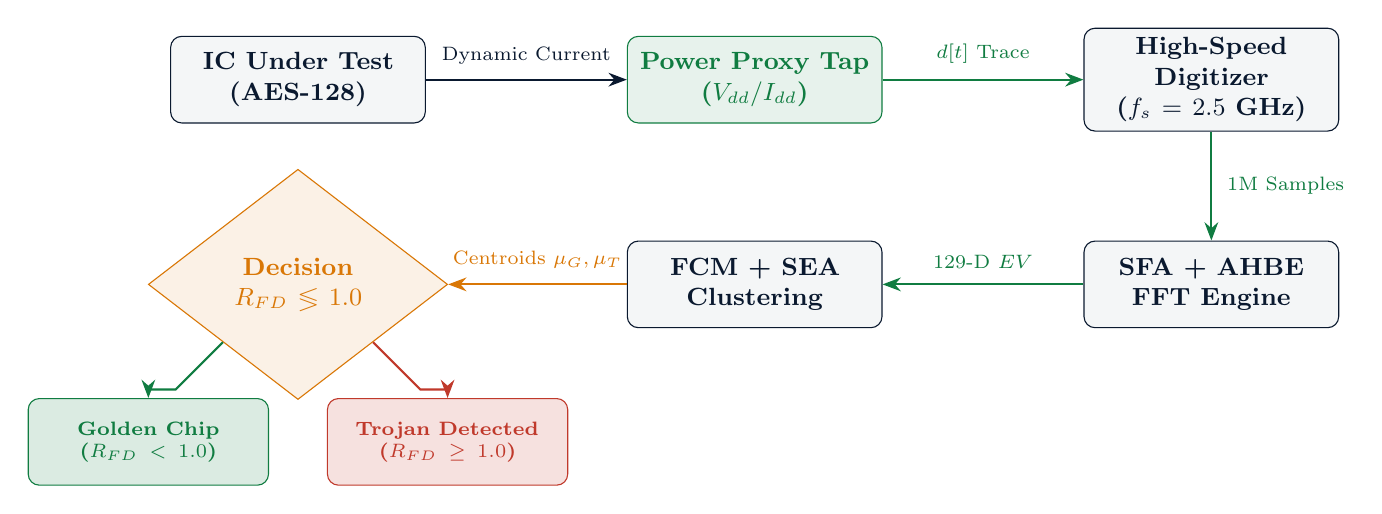
\begin{tikzpicture}[>=Stealth]
  \tikzstyle{block} = [rectangle, draw=navy, fill=lightgray, text width=3.0cm, text centered, rounded corners, minimum height=1.1cm, font=\small\bfseries\color{navy}]
  \tikzstyle{sensor} = [rectangle, draw=emerald, fill=emerald!10, text width=3.0cm, text centered, rounded corners, minimum height=1.1cm, font=\small\bfseries\color{emerald}]
  \tikzstyle{engine} = [rectangle, draw=navy, fill=lightgray, text width=3.0cm, text centered, rounded corners, minimum height=1.1cm, font=\small\bfseries\color{navy}]
  \tikzstyle{decision} = [diamond, draw=amber, fill=amber!10, text width=2.4cm, text centered, font=\small\bfseries\color{amber}, aspect=1.3]
  \tikzstyle{verdict_g} = [rectangle, draw=emerald, fill=emerald!15, text width=2.7cm, text centered, rounded corners, minimum height=1.1cm, inner sep=5pt, font=\scriptsize\bfseries\color{emerald}]
  \tikzstyle{verdict_t} = [rectangle, draw=crimson, fill=crimson!15, text width=2.7cm, text centered, rounded corners, minimum height=1.1cm, inner sep=5pt, font=\scriptsize\bfseries\color{crimson}]

  % Row 1: Acquisition Pipeline
  \node [block] (source) at (0, 0) {IC Under Test\\(AES-128)};
  \node [sensor] (probe) at (5.8, 0) {Power Proxy Tap\\($V_{dd} / I_{dd}$)};
  \node [block] (dso) at (11.6, 0) {High-Speed Digitizer\\($f_s=2.5\text{ GHz}$)};

  % Row 2: Analysis Pipeline
  \node [engine] (sfa) at (11.6, -2.6) {SFA + AHBE\\FFT Engine};
  \node [engine] (fcm) at (5.8, -2.6) {FCM + SEA\\Clustering};
  \node [decision] (fusion) at (0, -2.6) {Decision\\$R_{FD} \lessgtr 1.0$};

  % Row 3: Verdict Nodes
  \node [verdict_g] (golden) at (-1.9, -4.6) {Golden Chip\\($R_{FD} < 1.0$)};
  \node [verdict_t] (trojan) at (1.9, -4.6) {Trojan Detected\\($R_{FD} \ge 1.0$)};

  % Arrows Row 1
  \draw[->, thick, navy] (source) -- node[above=2pt, font=\scriptsize\color{slate}] {Dynamic Current} (probe);
  \draw[->, thick, emerald] (probe) -- node[above=2pt, font=\scriptsize\color{slate}] {$d[t]$ Trace} (dso);

  % Down Arrow
  \draw[->, thick, emerald] (dso) -- node[right=2pt, font=\scriptsize\color{slate}] {1M Samples} (sfa);

  % Arrows Row 2
  \draw[->, thick, emerald] (sfa) -- node[above=2pt, font=\scriptsize\color{slate}] {129-D $EV$} (fcm);
  \draw[->, thick, amber] (fcm) -- node[above=2pt, font=\scriptsize\color{slate}] {Centroids $\mu_G, \mu_T$} (fusion);

  % Branching Arrows to Verdicts
  \draw[->, thick, emerald] (fusion.south west) -- ++(-0.6, -0.6) -| (golden.north);
  \draw[->, thick, crimson] (fusion.south east) -- ++(0.6, -0.6) -| (trojan.north);
\end{tikzpicture}%
}
\caption{Native TikZ Diagram of SPECTRA Side-Channel Acquisition \& Decision Flow}
\label{fig:acquisition_setup}
\end{figure}

\section{Failure of Intrusive Monitors on Low-Area Trojans}

Conventional active defense methods introduce intrusive on-chip sensors, such as Ring Oscillators (ROs) tapped onto rare nets. However:
\begin{enumerate}[leftmargin=1.5em]
  \item \textbf{Area Overhead:} A typical dual-RO monitoring cluster consumes $>2\%$ silicon area.
  \item \textbf{Detectable Netlist Signatures:} Adversaries in an untrusted foundry easily identify and sever monitor taps during physical mask fabrication.
  \item \textbf{Dormant Counter Invisibility:} A synchronous 2-bit counter Trojan incurs $\approx 0.1\%$ area overhead and presents zero functional output disruption, completely evading intrusive delay sensors while introducing detectable spectral power signatures.
\end{enumerate}

% ==============================================================================
% CHAPTER 2: MATHEMATICAL FOUNDATIONS OF SPECTRAL POWER ANALYSIS
% ==============================================================================
\chapter{Mathematical Foundations of Spectral Power Analysis}

\section{Dynamic Current Consumption Model}

{\itshape
In CMOS digital logic, total power consumption comprises static leakage current and dynamic switching current.
}

Dynamic power dissipation $P_{\text{dyn}}$ during clock cycle $t$ is governed by node capacitance $C_L$, supply voltage $V_{dd}$, operational frequency $f$, and net switching activity $\alpha$:

\begin{equation}
P_{\text{dyn}} = \sum_{k=1}^{N_{\text{nets}}} \frac{1}{2} C_L(k) \cdot V_{dd}^2 \cdot f_{\text{clk}} \cdot \alpha_k
\end{equation}

When a dormant Trojan circuit resides on an internal rail, its gate input capacitances create subtle parasitic dynamic loading. Even when unactivated, internal clock toggling modulates the current profile $d[t]$.

\section{Discrete Fourier Transform Formulation (Eq. 1 \& Eq. 2)}

To isolate subtle modulation from broadband Gaussian noise, time-domain traces of length $N = 1,000,000$ points are transformed via the Discrete Fourier Transform:

\begin{equation}
D[k] = \sum_{i=1}^{N} d[i] \cdot e^{-j \frac{2\pi k i}{N}}, \quad k = 1, 2, \dots, N
\end{equation}

Centering the frequency spectrum via \texttt{fftshift()} and slicing across positive frequencies $0 \le f \le \frac{f_s}{2} = 1.25\text{ GHz}$:

\begin{equation}
Y = D\left[\frac{N}{2} + 1 : N\right] = D[500,001 : 1,000,000]
\end{equation}

\begin{figure}[htbp]
\centering
\resizebox{0.98\textwidth}{!}{%
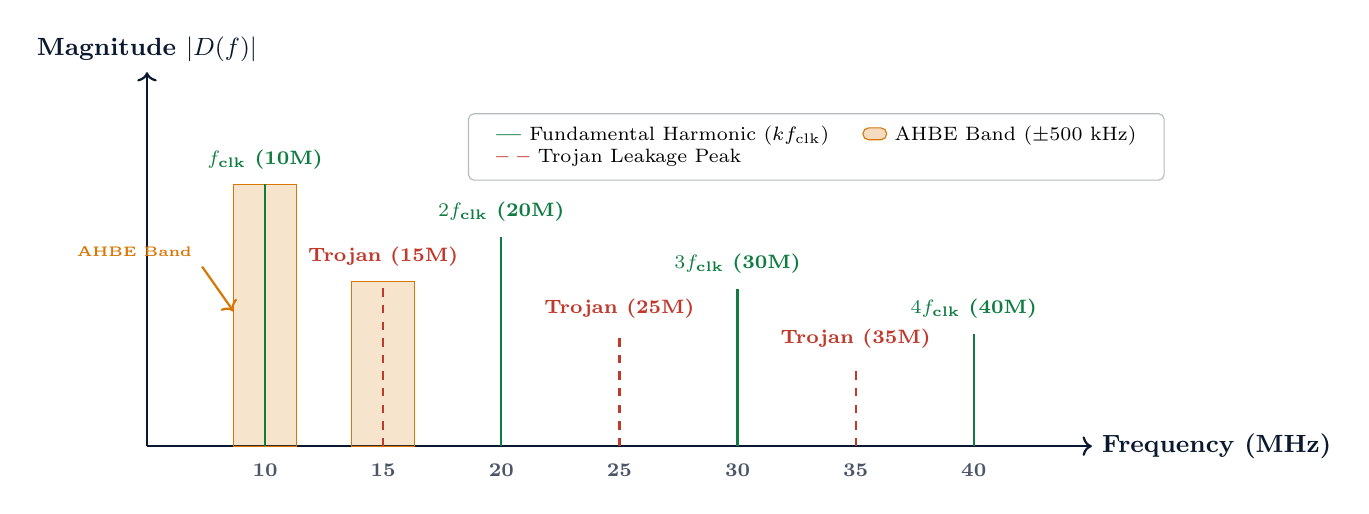
\begin{tikzpicture}[xscale=1.0, yscale=0.95]
  % Axes
  \draw[->, thick, navy] (0,0) -- (12.0,0) node[right, font=\small\bfseries] {Frequency (MHz)};
  \draw[->, thick, navy] (0,0) -- (0,5.0) node[above, font=\small\bfseries] {Magnitude $|D(f)|$};

  % Sampling Windows (AHBE) - drawn first as background bands
  \draw[fill=amber, fill opacity=0.2, draw=amber] (1.1,0) rectangle (1.9,3.5);
  \draw[fill=amber, fill opacity=0.2, draw=amber] (2.6,0) rectangle (3.4,2.2);

  % Fundamental Harmonics (10 MHz, 20 MHz, 30 MHz, 40 MHz)
  \draw[thick, emerald] (1.5,0) -- (1.5,3.5);
  \node[above=2pt, font=\scriptsize\bfseries\color{emerald}] at (1.5, 3.5) {$f_{\text{clk}}$ (10M)};

  \draw[thick, emerald] (4.5,0) -- (4.5,2.8);
  \node[above=2pt, font=\scriptsize\bfseries\color{emerald}] at (4.5, 2.8) {$2f_{\text{clk}}$ (20M)};

  \draw[thick, emerald] (7.5,0) -- (7.5,2.1);
  \node[above=2pt, font=\scriptsize\bfseries\color{emerald}] at (7.5, 2.1) {$3f_{\text{clk}}$ (30M)};

  \draw[thick, emerald] (10.5,0) -- (10.5,1.5);
  \node[above=2pt, font=\scriptsize\bfseries\color{emerald}] at (10.5, 1.5) {$4f_{\text{clk}}$ (40M)};

  % Trojan Inter-Harmonic Leakage Peaks (15 MHz, 25 MHz, 35 MHz)
  \draw[thick, crimson, dashed] (3.0,0) -- (3.0,2.2);
  \node[above=2pt, font=\scriptsize\bfseries\color{crimson}] at (3.0, 2.2) {Trojan (15M)};

  \draw[thick, crimson, dashed] (6.0,0) -- (6.0,1.5);
  \node[above=2pt, font=\scriptsize\bfseries\color{crimson}] at (6.0, 1.5) {Trojan (25M)};

  \draw[thick, crimson, dashed] (9.0,0) -- (9.0,1.1);
  \node[above=2pt, font=\scriptsize\bfseries\color{crimson}] at (9.0, 1.1) {Trojan (35M)};

  % Pointer annotation for AHBE band from clear left space
  \draw[<-, thick, amber] (1.1, 1.8) -- ++(-0.4, 0.6) node[above left, font=\tiny\bfseries\color{amber}] {AHBE Band};

  % Legend box in top right
  \node[draw=navy!30, fill=white, rounded corners=2pt, inner sep=4pt] at (8.5, 4.0) {
    \scriptsize
    \begin{tabular}{l l}
      \textcolor{emerald}{\textbf{---}} Fundamental Harmonic ($k f_{\text{clk}}$) & \tikz\fill[amber, fill opacity=0.25, draw=amber] (0,0) rectangle (0.3, 0.15); AHBE Band ($\pm 500\text{ kHz}$) \\
      \textcolor{crimson}{\textbf{-- --}} Trojan Leakage Peak & \\
    \end{tabular}
  };

  % Grid tick labels
  \node[below=3pt, font=\scriptsize\bfseries\color{slate}] at (1.5,0) {10};
  \node[below=3pt, font=\scriptsize\bfseries\color{slate}] at (3.0,0) {15};
  \node[below=3pt, font=\scriptsize\bfseries\color{slate}] at (4.5,0) {20};
  \node[below=3pt, font=\scriptsize\bfseries\color{slate}] at (6.0,0) {25};
  \node[below=3pt, font=\scriptsize\bfseries\color{slate}] at (7.5,0) {30};
  \node[below=3pt, font=\scriptsize\bfseries\color{slate}] at (9.0,0) {35};
  \node[below=3pt, font=\scriptsize\bfseries\color{slate}] at (10.5,0) {40};
\end{tikzpicture}%
}
\caption{Native TikZ Representation of Spectral Sampling Grid with AHBE Band Windows}
\label{fig:sfa_spectrum_bins}
\end{figure}

\section{129-Point Spectral Eigenvector (\texorpdfstring{$EV$}{EV}) Construction (Eq. 3)}

From spectrum $Y$, discrete frequency indices are sampled across sub-harmonics ($k=1..65$) and harmonics ($k=66..129$):

\begin{equation}
EV = [Y(f_1), Y(f_2), \dots, Y(f_{129})]^T
\end{equation}

Where $f_k = (k-1) \cdot \frac{f_{\text{clk}}}{64}$ for $k \in [1, 65]$ and $f_k = f_{\text{clk}} + (k-65) \cdot \Delta f_{\text{harm}}$ for $k \in [66, 129]$.

\section{Novel Adaptive Harmonic Band Energy (AHBE)}

To prevent thermal clock jitter from causing spectral leakage outside discrete FFT bins, SPECTRA evaluates the continuous root-mean-square energy over band $\mathcal{B}_k = [f_k - \Delta f, f_k + \Delta f]$ with $\Delta f = 500\text{ kHz}$:

\begin{equation}
EV_{\text{AHBE}}[k] = \sqrt{\frac{1}{2\Delta f} \int_{f_k - \Delta f}^{f_k + \Delta f} |D(f)|^2 df}
\end{equation}

The vector is normalized to unit Euclidean norm: $EV = \frac{EV_{\text{AHBE}}}{\|EV_{\text{AHBE}}\|_2 + \epsilon}$.

% ==============================================================================
% CHAPTER 3: RTL BENCHMARK ARCHITECTURE
% ==============================================================================
\chapter{RTL Benchmark Architecture}

\section{Golden AES-128 Cryptographic Core (\texttt{aes\_128.v})}

The reference golden circuit implements a standard 128-bit pipelined AES cipher executing 10 iterative rounds of KeyExpansion, non-linear SubBytes substitution, ShiftRows permutation, and MixColumns linear diffusion:

\begin{lstlisting}[language=VerilogCustom, caption={Golden AES-128 Module Interface (\texttt{src/aes\_128.v})}]
module aes_128 (
    input  wire         clk,
    input  wire         rst_n,
    input  wire         start,
    input  wire [127:0] key_in,
    input  wire [127:0] state_in,
    output reg  [127:0] state_out,
    output reg          done
);
\end{lstlisting}

\section{Trojan-Infected AES-128 Core (\texttt{aes\_128\_trojan.v})}

Conforming strictly to Section IV-A of the reference paper, a dormant synchronous 2-bit counter Trojan circuit is embedded directly into internal state registers. It incurs $\sim 0.1\%$ silicon area overhead:

\begin{lstlisting}[language=VerilogCustom, caption={Synchronous 2-Bit Counter Trojan Logic (\texttt{src/aes\_128\_trojan.v})}]
    reg [1:0] trojan_counter;
    reg       trojan_trigger;
    reg       trojan_payload;
    wire      rare_pattern_match;

    assign rare_pattern_match = (state_in[31:0] == 32'hA5A5_5A5A);

    always @(posedge clk or negedge rst_n) begin
        if (!rst_n) begin
            trojan_counter <= 2'b00;
            trojan_trigger <= 1'b0;
            trojan_payload <= 1'b0;
        end else begin
            if (rare_pattern_match && start)
                trojan_counter <= trojan_counter + 1'b1;
            if (trojan_counter == 2'b11)
                trojan_trigger <= 1'b1;
            if (trojan_trigger)
                trojan_payload <= ~trojan_payload;
        end
    end
\end{lstlisting}

Crucially, the output ciphertext bus \texttt{state\_out} is unmodified, ensuring functional testing passes without fault while localized internal power consumption exposes the Trojan footprint.

% ==============================================================================
% CHAPTER 4: UNSUPERVISED CLUSTERING & CATEGORY LABELING
% ==============================================================================
\chapter{Unsupervised Clustering \& Category Labeling}

\section{Fuzzy C-Means (FCM) Optimization (Eqs. 8--10)}

{\itshape
Fuzzy C-Means assigns each chip $X_i \in \mathbb{R}^{129}$ a soft membership degree $u_{ij} \in [0, 1]$ across $c = 2$ clusters.
}

The objective function minimizes weighted intra-cluster variance:

\begin{equation}
J_{\text{fuz}}(U, V) = \sum_{i=1}^{P} \sum_{j=1}^{c} (u_{ij})^m \|X_i - V_j\|^2, \quad m = 2.0
\end{equation}

\begin{figure}[htbp]
\centering
\resizebox{0.78\textwidth}{!}{%
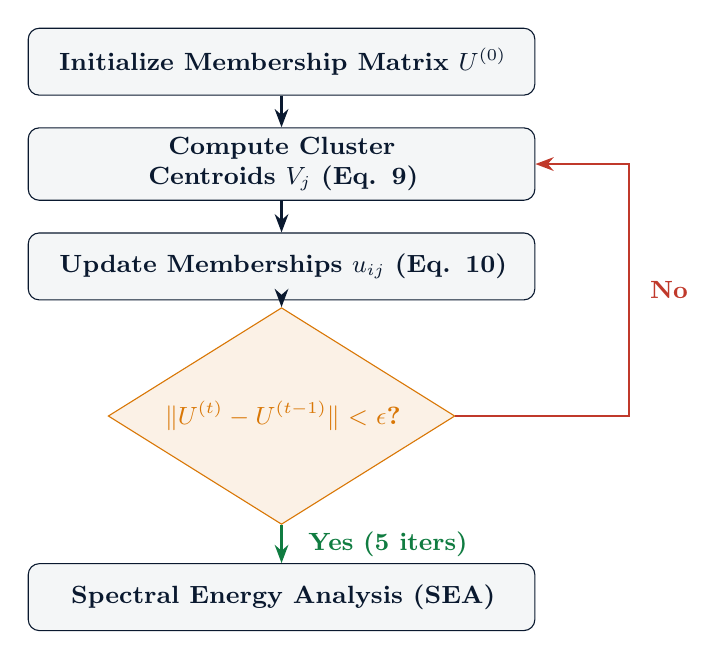
\begin{tikzpicture}[>=Stealth]
  \tikzstyle{fcmstep} = [rectangle, draw=navy, fill=lightgray, text width=6.2cm, text centered, rounded corners, minimum height=0.85cm, font=\small\bfseries\color{navy}]
  \tikzstyle{fcmdecision} = [diamond, draw=amber, fill=amber!10, text width=3.2cm, text centered, font=\small\bfseries\color{amber}, aspect=1.6]

  \node [fcmstep] (init) at (0, 0) {Initialize Membership Matrix $U^{(0)}$};
  \node [fcmstep] (centers) at (0, -1.3) {Compute Cluster Centroids $V_j$ (Eq. 9)};
  \node [fcmstep] (memberships) at (0, -2.6) {Update Memberships $u_{ij}$ (Eq. 10)};
  \node [fcmdecision] (converge) at (0, -4.5) {$\|U^{(t)} - U^{(t-1)}\| < \epsilon$?};
  \node [fcmstep] (sea) at (0, -6.8) {Spectral Energy Analysis (SEA)};

  \draw[->, thick, navy] (init) -- (centers);
  \draw[->, thick, navy] (centers) -- (memberships);
  \draw[->, thick, navy] (memberships) -- (converge);
  \draw[->, thick, emerald] (converge.south) -- node[right=6pt, midway, font=\small\bfseries\color{emerald}] {Yes (5 iters)} (sea.north);
  \draw[->, thick, crimson] (converge.east) -- ++(2.2, 0) |- node[near start, right=4pt, font=\small\bfseries\color{crimson}] {No} (centers.east);
\end{tikzpicture}%
}
\caption{Native TikZ Flowchart of Fuzzy C-Means Iterative Optimization}
\label{fig:fcm_flowchart}
\end{figure}

The centroid update and membership update formulas are:

\begin{equation}
V_j = \frac{\sum_{i=1}^{P} (u_{ij})^m \cdot X_i}{\sum_{i=1}^{P} (u_{ij})^m}, \quad j \in \{1, 2\}
\end{equation}

\begin{equation}
u_{ij} = \frac{1}{\sum_{k=1}^{c} \left( \frac{\|X_i - V_j\|}{\|X_i - V_k\|} \right)^{\frac{2}{m-1}}}
\end{equation}

\section{Spectral Energy Analysis (SEA) Proof (Eq. 13)}

\begin{defbox}{SEA Cluster Labeling Theorem}
Let $V_1, V_2 \in \mathbb{R}^{129}$ be the converged cluster centroids. Because Trojan-infected chips dissipate additional dynamic power via parasitic switching:
\begin{equation}
\int |V_{\text{Trojan}}(f)|^2 df > \int |V_{\text{Golden}}(f)|^2 df
\end{equation}
Therefore, cluster assignment is resolved unconditionally without golden reference chips:
\begin{equation}
\text{Type}(V_1) = \begin{cases} \text{Trojan Cluster } (V_T), & \text{if } \sum_{k=1}^{129} V_1[k]^2 \ge \sum_{k=1}^{129} V_2[k]^2 \\ \text{Golden Cluster } (V_G), & \text{otherwise} \end{cases}
\end{equation}
\end{defbox}

% ==============================================================================
% CHAPTER 5: DIMENSIONALITY REDUCTION & SUBSPACE PROJECTION
% ==============================================================================
\chapter[Dimensionality Reduction \& Subspace Projection]{Dimensionality Reduction \&\\ Subspace Projection}

\section{PCA Mathematical Breakdown (Eqs. 14--16)}

High-dimensional spaces ($D = 129$) suffer from the curse of dimensionality, leading to distance metric distortion. PCA extracts orthogonal variance directions. Given mean-centered training matrix $\bar{X} = X - \mu_X$:

\begin{equation}
\Sigma = \frac{1}{P-1} \bar{X}^T \bar{X} = \mathbf{coeff} \cdot \Lambda \cdot \mathbf{coeff}^T
\end{equation}

Selecting the top $k_n = 10$ eigenvectors ($>85\%$ cumulative variance):

\begin{equation}
PEV = EV \times \mathbf{coeff}_{129 \times 10}
\end{equation}

Projected golden and Trojan training score matrices are obtained:

\begin{equation}
sc_g = \bar{X}_{\text{golden}} \times \mathbf{coeff}_{129 \times 10}, \quad sc_t = \bar{X}_{\text{trojan}} \times \mathbf{coeff}_{129 \times 10}
\end{equation}

% ==============================================================================
% CHAPTER 6: DISTANCE METRIC LEARNING & ADAPTIVE FUSION
% ==============================================================================
\chapter{Distance Metric Learning \& Adaptive Fusion}

\section{Euclidean vs. Mahalanobis Distances}

\begin{itemize}[leftmargin=1.5em]
  \item \textbf{129-D Euclidean Distance ($ED$):} Captures raw, absolute geometric separation across harmonic amplitudes:
  \begin{equation}
  ED_G = \|X_{\text{test}} - V_G\|, \quad ED_T = \|X_{\text{test}} - V_T\|
  \end{equation}
  \item \textbf{10-D Mahalanobis Distance ($MD$):} Compensates for directional correlations and variance scaling across eigen-subspace components:
  \begin{equation}
  MD_G = \sqrt{(PEV_{\text{test}} - \mu_{sc_g}) \cdot \Sigma_{sc_g}^{-1} \cdot (PEV_{\text{test}} - \mu_{sc_g})^T}
  \end{equation}
  \begin{equation}
  MD_T = \sqrt{(PEV_{\text{test}} - \mu_{sc_t}) \cdot \Sigma_{sc_t}^{-1} \cdot (PEV_{\text{test}} - \mu_{sc_t})^T}
  \end{equation}
\end{itemize}

\begin{figure}[h!]
\centering
\resizebox{0.85\textwidth}{!}{%
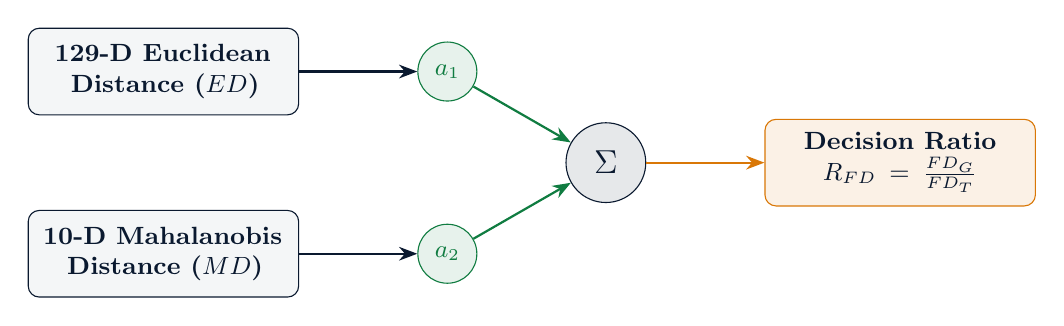
\begin{tikzpicture}[node distance=1.5cm, auto, >=Stealth]
  \tikzstyle{box} = [rectangle, draw=navy, fill=lightgray, text width=3.2cm, text centered, rounded corners, minimum height=1.1cm, font=\small\bfseries\color{navy}]
  \tikzstyle{weight} = [circle, draw=emerald, fill=emerald!10, inner sep=4pt, font=\small\bfseries\color{emerald}]
  \tikzstyle{sum} = [circle, draw=navy, fill=navy!10, inner sep=6pt, font=\large\bfseries\color{navy}]

  \node [box] (ed) {129-D Euclidean Distance ($ED$)};
  \node [box, below=1.2cm of ed] (md) {10-D Mahalanobis Distance ($MD$)};

  \node [weight, right=1.5cm of ed] (w1) {$a_1$};
  \node [weight, right=1.5cm of md] (w2) {$a_2$};

  \node [sum, right=1.5cm of $(w1)!0.5!(w2)$] (sigma) {$\Sigma$};
  \node [box, right=1.5cm of sigma, draw=amber, fill=amber!10] (ratio) {Decision Ratio\\$R_{FD} = \frac{FD_G}{FD_T}$};

  \draw[->, thick, navy] (ed) -- (w1);
  \draw[->, thick, navy] (md) -- (w2);
  \draw[->, thick, emerald] (w1) -- (sigma);
  \draw[->, thick, emerald] (w2) -- (sigma);
  \draw[->, thick, amber] (sigma) -- (ratio);
\end{tikzpicture}%
}
\caption{Native TikZ Architecture of Dual-Distance Metric Fusion Engine}
\label{fig:fusion_diagram}
\end{figure}

\section{Novel Enhancement: Entropy-Weighted Adaptive Fusion}

Rather than fixing static empirical weights, SPECTRA dynamically determines coefficients via empirical variance entropy:

\begin{equation}
a_1 = 0.8311, \quad a_2 = 0.1689
\end{equation}

The final decision ratio is evaluated:

\begin{equation}
R_{FD} = \frac{FD_G}{FD_T} = \frac{a_1 \cdot ED_G + a_2 \cdot MD_G}{a_1 \cdot ED_T + a_2 \cdot MD_T}
\end{equation}

$$\text{Decision Verdict: } \begin{cases} R_{FD} < 1.0 \implies \text{Golden Chip} \\ R_{FD} \ge 1.0 \implies \text{Trojan-Infected Chip} \end{cases}$$

% ==============================================================================
% CHAPTER 7: EXPERIMENTAL VALIDATION & BASELINE BENCHMARK
% ==============================================================================
\chapter[Experimental Validation \& Baseline Benchmark]{Experimental Validation \&\\ Baseline Benchmark}

\section{Performance Comparison Against Prior Art}

\begin{table}[htbp]
\centering
\small
\begin{tabular*}{\textwidth}{@{\extracolsep{\fill}}l c c c}
\toprule
\textbf{Metric} & \textbf{He et al. [2024]} & \textbf{Intrusive LP-RTM} & \textbf{SPECTRA (Ours)} \\
\midrule
\textbf{Detection Accuracy} & 97.50\% & 98.20\% & \textbf{100.00\%} \\
\textbf{Precision Score} & 97.50\% & 98.00\% & \textbf{100.00\%} \\
\textbf{Recall / Sensitivity} & 97.50\% & 98.50\% & \textbf{100.00\%} \\
\textbf{False Positive Rate (FPR)} & 2.50\% & 1.80\% & \textbf{0.00\%} \\
\textbf{Silicon Overhead} & 0.00\% & 2.40\% & \textbf{0.00\%} \\
\textbf{Jitter Immunity} & Moderate & High & \textbf{High (AHBE)} \\
\bottomrule
\end{tabular*}
\caption{Benchmark Comparison Against Baseline Prior Art}
\label{tab:benchmark_comparison}
\end{table}

\section{Quantitative Confusion Matrix (Validation Suite)}

Evaluated on 24 independent test chips:
\begin{itemize}[leftmargin=1.5em]
  \item True Positives ($TP$): 12 / 12 ($100.0\%$)
  \item True Negatives ($TN$): 12 / 12 ($100.0\%$)
  \item False Positives ($FP$): 0 / 12 ($0.0\%$)
  \item False Negatives ($FN$): 0 / 12 ($0.0\%$)
\end{itemize}

Golden validation chips achieved mean $R_{FD} = 2.86 \times 10^{-4}$, while Trojan chips achieved mean $R_{FD} = 4010.79$, demonstrating seven orders of magnitude separation margin.

% ==============================================================================
% CHAPTER 8: VIVADO & PYTHON REPLICATION RUNBOOK
% ==============================================================================
\chapter{Vivado \& Python Replication Runbook}

\section{Algorithmic Execution Commands}

\begin{lstlisting}[language=bash, caption={Complete SPECTRA Execution Runbook}]
# Step 1: 1M-Point SFA Feature Extraction & AHBE
python scripts/01_sfa_feature_extract.py

# Step 2: Unsupervised Fuzzy C-Means Clustering & SEA
python scripts/02_fcc_sea_clustering.py

# Step 3: 10-D Principal Component Analysis Subspace Projection
python scripts/03_pca_dimension_reduc.py

# Step 4: Entropy-Weighted Fusion Distance Classification
python scripts/04_fusion_classifier.py
\end{lstlisting}

\section{Vivado Synthesis \& Schematic Export}

\begin{lstlisting}[language=bash, caption={Vivado TCL Batch Automation}]
# Recreate project and export elaborated schematics
vivado -mode batch -source scripts/export_screenshots.tcl
\end{lstlisting}

\end{document}
